\documentclass{article}

\usepackage{graphicx}
\usepackage{authblk}
\usepackage{listings}
\usepackage{xcolor}
\usepackage[a4paper,
            bindingoffset=0.2in,
            left=0.5in,
            right=0.5in,
            top=0.5in,
            bottom=0.5in,
            footskip=.25in]{geometry}

\definecolor{mGreen}{rgb}{0,0.6,0}
\definecolor{mGray}{rgb}{0.5,0.5,0.5}
\definecolor{mPurple}{rgb}{0.58,0,0.82}
\definecolor{backgroundColour}{rgb}{0.95,0.95,0.92}

\lstdefinestyle{CStyle}{
    backgroundcolor=\color{backgroundColour},   
    commentstyle=\color{mGreen},
    keywordstyle=\color{magenta},
    numberstyle=\tiny\color{mGray},
    stringstyle=\color{mPurple},
    basicstyle=\footnotesize,
    breakatwhitespace=false,         
    breaklines=true,                 
    captionpos=b,                    
    keepspaces=true,                 
    numbers=left,                    
    numbersep=5pt,                  
    showspaces=false,                
    showstringspaces=false,
    showtabs=false,                  
    tabsize=2,
    language=C
}


\title{Assignment 4: Functions}
\author{Cody Raposa}
\affil{ELEC2850 Microcontrollers Using C Programming}

\begin{document}
\maketitle
\begin{flushleft}
  \section{Part 1}
  \begin{figure}[!h]
    \begin{centering}
      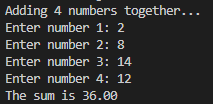
\includegraphics[scale=1]{P1_output.png}
      \caption{Test cases for Part 1}
    \end{centering}
  \end{figure}
  \lstinputlisting[style=CStyle]{P1.c}
  \newpage
  \section{Part 3}
  \begin{figure}[!h]
    \begin{centering}
      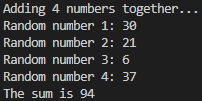
\includegraphics[scale=1]{P3_output.png}
      \caption{Test cases for Part 3}
    \end{centering}
  \end{figure}
  \lstinputlisting[style=CStyle]{P3.c}
  \section{Part 4}
  \begin{figure}[!h]
    \begin{centering}
      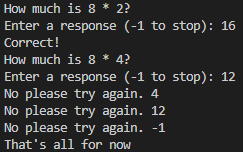
\includegraphics[scale=1]{P4_output.png}
      \caption{Test cases for Part 4}
    \end{centering}
  \end{figure}
  \newpage
  \lstinputlisting[style=CStyle]{P4.c}
  \newpage
  \section{Part 5 Problem Statement}
  Using the code from part 4, modify it to vary the resssponses for a correct and incorrect response, using functions.
  %\section{Assumptions}
  %\section{Algorithm}
  \section{Analysis}
  \subsection{Inputs}
  Answer (int)
  %\section{Pseudocode}
  \section{Flowchart}
    \begin{figure}[!h]
      \begin{centering}
        \includegraphics[scale=0.5]{P5_Flowchart.png}
        \caption{Flowchart for Q2}
      \end{centering}
    \end{figure}
    \newpage
  \section{Output}
  \begin{figure}[!h]
    \begin{centering}
      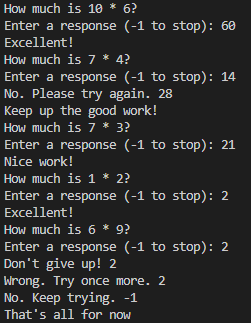
\includegraphics[scale=1]{P5_output.png}
      \caption{A test case for the program}
    \end{centering}
  \end{figure}
  \section{Code}
  \lstinputlisting[style=CStyle]{P5.c}
\end{flushleft}
\end{document}